\documentclass[a4paper]{article}

\def\npart {PK/PD Foundations}
\def\nterm {Direct effect models}
\def\nyear {2026}
\def\nlecturer {Mager and Straubinger; Levy; Wagner}
\def\ncourse {Gerhard Levy: direct effect model 的第一性洞察}
\def\ncoursehead {Levy direct effect}
\def\nauthor {NanFangHong}

\RequirePackage{etex}
\makeatletter
\ifx \npart \undefined
  \def\npart{PK/PD Notes}
\fi
\ifx \nterm \undefined
  \def\nterm{Reading notes}
\fi
\ifx \nyear \undefined
  \def\nyear{\the\year}
\fi
\ifx \nlecturer \undefined
  \def\nlecturer{the source literature}
\fi
\ifx \nauthor \undefined
  \def\nauthor{NanFangHong}
\fi
\ifx \ncourse \undefined
  \def\ncourse{Pharmacology Reading Note}
\fi
\ifx \ncoursehead \undefined
  \def\ncoursehead{\ncourse}
\fi

\author{Based on \nlecturer \\\small Notes taken by \nauthor}
\date{\nterm\ \nyear}
\title{\npart\ --- \ncourse}

\usepackage{amsfonts}
\usepackage{amsmath}
\usepackage{amssymb}
\usepackage{amsthm}
\usepackage{booktabs}
\usepackage{caption}
\usepackage{enumitem}
\usepackage{fancyhdr}
\usepackage{fontspec}
\usepackage{graphicx}
\usepackage{iftex}
\usepackage{mathtools}
\usepackage{microtype}
\usepackage{siunitx}
\usepackage{tabularx}
\usepackage{tikz}
\usepackage{xcolor}
\usepackage{xurl}
\usepackage{xeCJK}

\IfFontExistsTF{Latin Modern Roman}{
  \setmainfont[Ligatures=NoCommon]{Latin Modern Roman}
}{}

\IfFontExistsTF{Noto Serif CJK SC}{
  \setCJKmainfont{Noto Serif CJK SC}
}{
  \IfFontExistsTF{Songti SC}{
    \setCJKmainfont{Songti SC}
  }{
    \IfFontExistsTF{PingFang SC}{
      \setCJKmainfont{PingFang SC}
    }{}
  }
}

\usepackage[hidelinks,unicode,breaklinks=true]{hyperref}
\hypersetup{
  pdfauthor={\nauthor},
  pdfsubject={\npart\ - \ncourse},
  pdftitle={\npart\ - \ncourse},
  pdfkeywords={PK PD pharmacology reading notes \ncourse}
}

\pagestyle{fancyplain}
\lhead{\emph{\nouppercase{\leftmark}}}
\rhead{
  \ifnum\thepage=1
  \else
    \npart\ \ncoursehead
  \fi}

\theoremstyle{definition}
\newtheorem*{aim}{Aim}
\newtheorem*{assumption}{Assumption}
\newtheorem*{defi}{Definition}
\newtheorem*{eg}{Example}
\newtheorem*{notation}{Notation}
\newtheorem*{question}{Question}
\newtheorem*{remark}{Remark}
\newtheorem*{warning}{Warning}

\theoremstyle{plain}
\newtheorem{nthm}{Theorem}[section]
\newtheorem{nprop}[nthm]{Proposition}

\renewcommand{\labelitemi}{--}
\renewcommand{\labelitemii}{$\circ$}
\renewcommand{\labelenumi}{(\roman{*})}

\let\stdsection\section
\renewcommand\section{\newpage\stdsection}

\newcommand{\dd}{\mathop{}\!\mathrm{d}}
\newcommand{\Emax}{E_{\max}}
\newcommand{\pksym}[1]{\ifmmode\text{\textit{#1}}\else\textit{#1}\fi}
\newcommand{\pklab}[1]{\mathrm{#1}}
\newcommand{\ECfifty}{\pksym{EC}_{50}}
\newcommand{\term}[1]{\emph{#1}}
\makeatother


\begin{document}
\maketitle
{\small
  \noindent\textbf{Reading motive}\\
  这篇笔记记录 Gerhard Levy 对 direct effect model 的一个漂亮洞察：当药物按一阶消除下降，而效应在局部近似为 log concentration 的线性函数时，药效的消失速度会变成一个近似常数。\hspace*{\fill}[Levy]

  \vspace{5pt}
  \noindent\textbf{Core image}\\
  Pharmacodynamics 在这里不是一个神秘黑箱，而是把 ``concentration falls with time'' 和 ``effect changes with concentration'' 接在一起。The bridge is almost just the chain rule.\hspace*{\fill}[chain rule]

  \vspace{5pt}
  \noindent\textbf{Use for later notes}\\
  这个小模型会作为之后阅读 indirect response、effect compartment、turnover model 和 mechanism-based PK-PD 的基准坐标。\hspace*{\fill}[baseline]
}

\tableofcontents

\section{文献入口}

\subsection{Context}

Mager and Straubinger 在回顾 William Jusko 对 PK-PD 建模的贡献时，把 direct effect model 放在一组基础模型的起点位置：最简单的情形是，血液或血浆中的 drug concentration time-course 直接控制即时药效。这个框架适合描述一些相对贴近血液的响应，例如 enzyme activity 或 cell activity 的变化 \cite{mager2024jusko}。

\begin{remark}
  我读到这里的兴趣点不是 ``direct effect model 很简单''，而是 Levy 怎样把简单模型变成一个可计算的直觉：PK 的下降速率和 PD 曲线的斜率相乘，就能预测 response 消失的速度。
\end{remark}

\subsection{The question}

直接效应模型真正问的是：
\[
  C(t) \longrightarrow E(t)
\]
这个箭头能不能近似为没有明显 delay、没有 hidden turnover、也不需要 effect compartment 的即时映射？

如果答案是 yes，那么模型的最小版本就不是先去追踪 receptor、gene expression 或 downstream biomarkers，而是先问：

\begin{question}
  当 plasma concentration 随时间下降时，effect 会沿着 concentration--effect curve 以什么速度滑下来？
\end{question}

\section{Levy's move}

\subsection{Local linearity}

Levy 的洞察可以从一个局部线性图像开始。假设在我们关心的浓度范围内，效应和 log concentration 的关系近似为一条直线：
\[
  E \approx a + m \log C.
\]
这里的 \(m\) 是 concentration--effect curve 在这个局部范围的斜率。它回答的是：\(\log C\) 每下降一点，effect 会下降多少？

另一方面，如果 drug concentration 服从一阶消除，
\[
  C(t)=C_0e^{-kt},
\]
那么 \(\log C\) 会随时间近似线性下降：
\[
  \log C(t)=\log C_0-kt.
\]

\subsection{A chain-rule view}

把两件事接起来，就是 Levy insight 的核心：
\[
  \frac{\dd E}{\dd t}
  =
  \frac{\dd E}{\dd \log C}
  \cdot
  \frac{\dd \log C}{\dd t}
  \approx
  m \cdot (-k).
\]

所以 response 的 loss rate 可以近似看成常数：
\[
  -\frac{\dd E}{\dd t}\approx m k.
\]

This is why a first-order PK process can generate an apparently zero-order loss of pharmacological response. 注意这里的 zero-order 不是说 drug elimination 变成零级，而是说 response decline 在这个局部线性区域里接近 constant rate。

\begin{remark}
  对我来说，这个地方很美：PK 给了时间轴上的速度，PD 给了曲线上的斜率；两者相乘，就把 ``concentration falling'' 翻译成 ``effect fading''。
\end{remark}

\section{Diagram}

\subsection{我的图}

下面这张图把 \(m\) 和 \(k\) 的关系画成一个几何乘法。竖直方向是 effect \(E\)，横向是 \(\log[C]\)，斜向箭头表示 time \(t\)。黄色段可以理解为 \(\log[C]\) 的变化，青色段是 effect 的变化，红色段是沿时间方向看到的 response loss。

\begin{center}
\tikzset{every picture/.style={line width=0.75pt}}
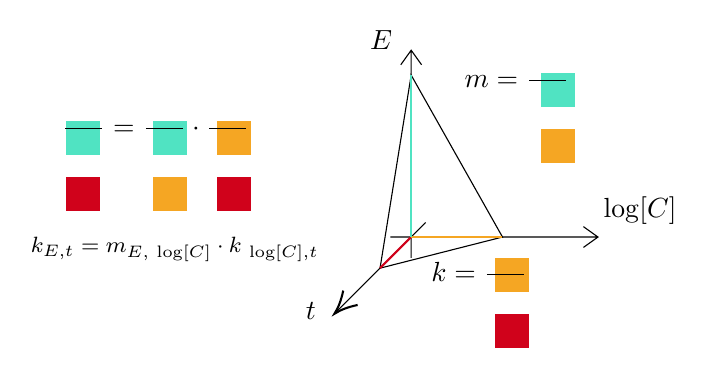
\begin{tikzpicture}[x=0.75pt,y=0.75pt,yscale=-1,xscale=1]
%Shape: Axis 2D [id:dp46038734449035423]
\draw  (203,121) -- (303,121)(213,31) -- (213,131) (296,116) -- (303,121) -- (296,126) (208,38) -- (213,31) -- (218,38)  ;
%Straight Lines [id:da2910877558581151]
\draw    (220,114) -- (177.41,156.59) ;
\draw [shift={(176,158)}, rotate = 315] [color={rgb, 255:red, 0; green, 0; blue, 0 }  ][line width=0.75]    (10.93,-4.9) .. controls (6.95,-2.3) and (3.31,-0.67) .. (0,0) .. controls (3.31,0.67) and (6.95,2.3) .. (10.93,4.9)   ;
%Shape: Right Triangle [id:dp47255015484811036]
\draw   (213,43) -- (257,121) -- (213,121) -- cycle ;
%Straight Lines [id:da19915034912265495]
\draw    (257,121) -- (198,136) ;
%Straight Lines [id:da4663359203301414]
\draw    (213,43) -- (198,136) ;
%Straight Lines [id:da26174075489503945]
\draw [color={rgb, 255:red, 208; green, 2; blue, 27 }  ,draw opacity=1 ][line width=0.75]    (198,136) -- (213,121) ;
%Straight Lines [id:da06543063184938513]
\draw [color={rgb, 255:red, 245; green, 166; blue, 35 }  ,draw opacity=1 ][line width=0.75]    (213,121) -- (257,121) ;
%Straight Lines [id:da21095721352816466]
\draw [color={rgb, 255:red, 80; green, 227; blue, 194 }  ,draw opacity=1 ][line width=0.75]    (213,121) -- (213,43) ;
%Shape: Square [id:dp15863092101349274]
\draw  [draw opacity=0][fill={rgb, 255:red, 80; green, 227; blue, 194 }  ,fill opacity=1 ] (275.5,42) -- (292,42) -- (292,58.5) -- (275.5,58.5) -- cycle ;
%Shape: Square [id:dp32909472986993715]
\draw  [draw opacity=0][fill={rgb, 255:red, 245; green, 166; blue, 35 }  ,fill opacity=1 ] (275.5,69) -- (292,69) -- (292,85.5) -- (275.5,85.5) -- cycle ;
%Shape: Square [id:dp36722223025287404]
\draw  [draw opacity=0][fill={rgb, 255:red, 245; green, 166; blue, 35 }  ,fill opacity=1 ] (253.5,131) -- (270,131) -- (270,147.5) -- (253.5,147.5) -- cycle ;
%Shape: Square [id:dp5134883252781336]
\draw  [draw opacity=0][fill={rgb, 255:red, 208; green, 2; blue, 27 }  ,fill opacity=1 ] (253.5,158) -- (270,158) -- (270,174.5) -- (253.5,174.5) -- cycle ;
%Shape: Square [id:dp3956700851727647]
\draw  [draw opacity=0][fill={rgb, 255:red, 80; green, 227; blue, 194 }  ,fill opacity=1 ] (88.5,65) -- (105,65) -- (105,81.5) -- (88.5,81.5) -- cycle ;
%Shape: Square [id:dp8062918601304804]
\draw  [draw opacity=0][fill={rgb, 255:red, 245; green, 166; blue, 35 }  ,fill opacity=1 ] (88.5,92) -- (105,92) -- (105,108.5) -- (88.5,108.5) -- cycle ;
%Shape: Square [id:dp1898873333514236]
\draw  [draw opacity=0][fill={rgb, 255:red, 245; green, 166; blue, 35 }  ,fill opacity=1 ] (119.5,65) -- (136,65) -- (136,81.5) -- (119.5,81.5) -- cycle ;
%Shape: Square [id:dp5763068272795581]
\draw  [draw opacity=0][fill={rgb, 255:red, 208; green, 2; blue, 27 }  ,fill opacity=1 ] (119.5,92) -- (136,92) -- (136,108.5) -- (119.5,108.5) -- cycle ;
%Shape: Square [id:dp6311468107674447]
\draw  [draw opacity=0][fill={rgb, 255:red, 80; green, 227; blue, 194 }  ,fill opacity=1 ] (46.5,65) -- (63,65) -- (63,81.5) -- (46.5,81.5) -- cycle ;
%Shape: Square [id:dp16267102140639023]
\draw  [draw opacity=0][fill={rgb, 255:red, 208; green, 2; blue, 27 }  ,fill opacity=1 ] (46.5,92) -- (63,92) -- (63,108.5) -- (46.5,108.5) -- cycle ;

% Text Node
\draw (161,151.4) node [anchor=north west][inner sep=0.75pt]    {$t$};
% Text Node
\draw (300,100.4) node [anchor=north west][inner sep=0.75pt]    {$\ \log[ C]$};
% Text Node
\draw (192,20.4) node [anchor=north west][inner sep=0.75pt]    {$E$};
% Text Node
\draw (237.5,41.9) node [anchor=north west][inner sep=0.75pt]    {$m=\frac{\ \ \ \ }{}$};
% Text Node
\draw (221.5,131.9) node [anchor=north west][inner sep=0.75pt]    {$k=\frac{\ \ \ \ }{}$};
% Text Node
\draw (43.5,64.9) node [anchor=north west][inner sep=0.75pt]    {$\frac{\ \ \ \ }{} =\frac{\ \ \ \ }{} \cdot \frac{\ \ \ \ }{}$};
% Text Node
\draw (28.5,119.9) node [anchor=north west][inner sep=0.75pt]  [font=\footnotesize]  {$k_{E,t} =m_{E,\ \log[ C]} \cdot k_{\ \log[ C] ,t}$};
\end{tikzpicture}

\captionof{figure}{我的 Levy direct effect sketch: response decline is the product of a PD slope and a PK decline rate.}
\end{center}

\subsection{What the sketch says}

图里的乘法不是代数炫技，而是一个 modeling stance：

\begin{itemize}[leftmargin=2em]
  \item \(m_{E,\log C}\) 描述 pharmacological sensitivity：effect 对 concentration 变化有多敏感。
  \item \(k_{\log C,t}\) 描述 PK speed：\(\log C\) 沿时间下降得多快。
  \item \(k_{E,t}\) 是我们在实验里真正看到的 response fading speed。
\end{itemize}

如果 response decline 很快，可能是 clearance 很快，也可能是 concentration--effect curve 很陡；如果 response 持续很久，可能是 \(C(t)\) 长时间高于 minimum effective concentration，也可能是 slope 很平。这个图提醒我不要把 duration 只归因于 half-life。

\section{Duration as threshold crossing}

\subsection{Minimum effective concentration}

Levy 的想法也自然导向一个经典判断：很多 drug effects 的 duration 主要由 plasma concentration 保持在某个 minimum effective concentration 之上的时间决定。这个阈值可以是 \(EC_{10}\)、\(IC_{10}\)，或者更一般的 \(\mathrm{MEC}\)。

在一阶消除下，如果
\[
  C(t)=C_0e^{-kt},
\]
那么 effect duration 可以粗略写成
\[
  T_{\mathrm{effect}}
  \approx
  \frac{1}{k}\log\!\left(\frac{C_0}{\mathrm{MEC}}\right).
\]

这个式子非常 accessible：dose 改变 \(C_0\)，clearance/elimination 改变 \(k\)，而 pharmacodynamic threshold 决定什么时候 effect ends。

\subsection{Limits}

这个 direct effect intuition 有边界。只要出现明显 hysteresis、biophase distribution delay、receptor turnover、signal transduction 或 homeostatic feedback，\(C(t)\rightarrow E(t)\) 的即时映射就会变得不够。那时需要 effect compartment、indirect response 或更 mechanism-based 的模型。

\section{Wagner's extension}

\subsection{From line to curve}

Levy 的局部线性图像解释了一个很干净的现象：为什么 effect 可以近似匀速消失。John Wagner 后来把这个思路推进到更完整的 concentration--response curve：用 nonlinear Hill function 或 Emax-type relation，把 PK 产生的 \(C(t)\) 投影到完整的 response profile \cite{wagner1968response}。

一个常见形式是
\[
  E(C)=E_0+\frac{\Emax C^\gamma}{EC_{50}^{\gamma}+C^\gamma}.
\]

这时 \(m\) 不再是全程固定的常数，而是曲线在每个浓度点的 local slope。换句话说，Levy 的 \(m\cdot k\) 仍然像一个局部指南针，只是 \(m\) 会随着 \(C\) 的位置而改变。

\subsection{My takeaway}

我想把这条线索记成一句话：

\begin{quote}
  Direct effect modeling starts when PK supplies the clock, PD supplies the curve, and their product supplies the time-course of response.
\end{quote}

这也是为什么 Gerhard Levy 会被称为 pharmacodynamics 的奠基者之一：他不是只说 ``effect follows concentration''，而是把这个跟随关系变成了可以推导、可以画图、可以预测 duration 的定量语言 \cite{levy1966kinetics,mager2024jusko}。

\bibliographystyle{plain}
\bibliography{../refs/pharmacology}

\end{document}
